\documentclass[../thesis.tex]{subfiles}
\graphicspath{{../gfx/}{gfx/}}
\begin{document}
\begin{flushleft}
\fontsize{12pt}{30pt}\selectfont

\vspace*{6mm}

\begin{tabular}{l l}
  \begin{minipage}{4cm}
    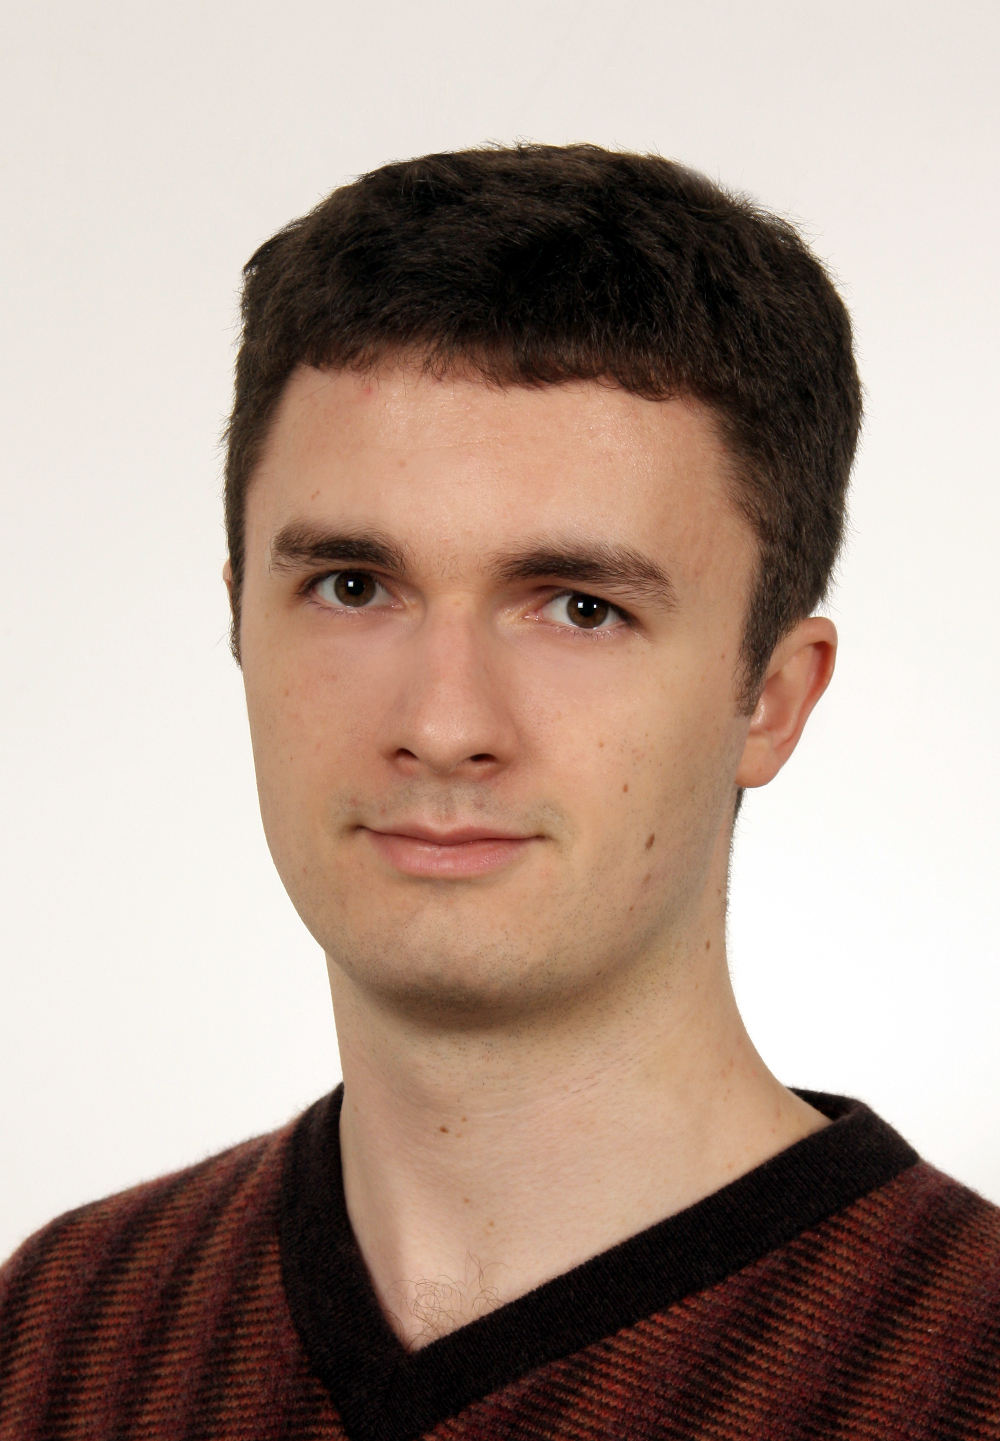
\includegraphics[height=4.5cm]{face.jpg}
  \end{minipage}
  &
  \begin{minipage}{15cm}
    Kierunek: \hspace{15mm} Informatyka

    Specjalność: \hspace{10mm} Inżynieria Systemów Informatycznych

    Data urodzenia: \hspace{51mm} 12.01.1990

    Data rozpoczęcia studiów: \hspace{33mm} 01.10.2009
  \end{minipage}
\end{tabular} 


\vspace{1.5cm}

\begin{center}
Życiorys
\end{center}
Urodziłem się 12 stycznia 1990 r. w Warszawie. Uczęszczałem do Szkoły Podstawowej Nr 218 im. Michała Kajki oraz Nr 173 im. Górników Polskich w Warszawie. Ukończyłem Gimnazjum Nr 119 im. Józefa Piłsudskiego oraz Liceum Nr 14 im. Stanisława Staszica w Warszawie. W 2009 r. zostałem studentem Wydziału Elektroniki i Technik Informacyjnych Politechniki Warszawskiej. W 2012 r. semestr studiów spędziłem na uczelni zagranicznej Kungliga Tekniska Hogskolan w Szwecji.
\vspace{1cm}

\fontsize{12pt}{14pt}\selectfont
\hspace*{100mm}..................................................... \\
\hspace*{115mm}Podpis studenta
\vspace*{1cm}

\fontsize{12pt}{30pt}\selectfont
EGZAMIN DYPLOMOWY \\
Złożył egzamin dyplomowy w dniu ............................................................................... 20\_\_ r \\

z wynikiem .................................................................................................................................

Ogólny wynik studiów: ..............................................................................................................

Dodatkowe wnioski i uwagi Komisji: ........................................................................................

.....................................................................................................................................................

.....................................................................................................................................................

\end{flushleft}
\pagestyle{empty}
\cleardoublepage 
\end{document}
